% -----------------------------------------------------------------------------
\section{Complementary Standards}
\label{sec:complementaryStandards}
% -----------------------------------------------------------------------------
\subsection{Adding Provenance with PROV-O}
\label{sec:provenance}
\label{sec:wasGeneratedBys}

The PROV-O ontology (\url{https://www.w3.org/TR/prov-o/}) defines a complementary data model that is leveraged by SBOL to describe provenance. Provenance is central to a range of workflow management, quality control, and attribution tasks within the Synthetic Biology design process. Tracking attribution and derivation of one resource from another is paramount for managing intellectual property purposes. Source designs are often modified in systematic ways to generate derived designs, for example, by applying codon optimization or systematically removing all of a class of restriction enzyme sites.  Documenting the transformation used, and any associated parameters, makes this explicit and potentially allows the process to be reproduced systematically. If a design has been used within other designs, and is later found to be defective, it is paramount that all uses of it, including uses of edited versions of the design, can be identified, and ideally replaced with a non-defective alternative. When importing data from external sources, it is important not only to attribute the original source (for example, GenBank), but also the tool used to perform the import, as this may have made arbitrary choices as to how to represent the source knowledge as SBOL. All these activities have in common that it is necessary to track what resource, and what transformation process was applied by whom to derive an SBOL design.

This section describes a minimal subset of PROV-O terms and classes that may be used by SBOL tools to support representation of provenance\footnote{We thank Dr Paolo Missier from the School of Computing Science, Newcastle University for discussions regarding the use of PROV-O.}. Although the full-set of PROV-O terms can be used in SBOL documents, a subset of PROV-O is adopted as a best practice. It is advised that SBOL tools should at least understand this subset, defined in \ref{uml:provenance}. Providers of provenance information are free to make use of more of PROV-O than is described here. It is acceptable for tools that understand more than this subset to use as much as they are able. Tools that only understand this subset must treat any additional data as annotations. Tools that are not aware of SBOL provenance at all MUST maintain and provide access to this information as annotations. This specification does not state what the newly added properties must point to. As long as they are resources that are consistent with the PROV-O property domains, they are legal. For example, a \sbol{Component} may be derived from another \sbol{Component}, but it would probably not make sense for it to be derived from a \sbol{Collection}.

The most basic and general type of provenance relationship can be represented using the \prov{wasDerivedFrom} property. This relationship describes derivation of an SBOL entity from another. 
Any \sbol{Identified} object may be annotated with this property. More specific provenance relationships can also be defined using PROV-O, such as \prov{wasGeneratedBy}. Generation of a new object is defined by the W3C PROV-O specification as follows:
\begin{quote}
	...the completion of production of a new entity by an activity. This entity did not exist before generation and becomes available for usage after this generation.
\end{quote}
These relationships are leveraged in SBOL tooling for describing multi-stage synthetic biology workflows.

Synthetic biology workflows may involve multiple stages, multiple users, multiple organizations, and interdisciplinary collaborations. These workflows can be described using four core PROV-O classes: \texttt{Entity}, \texttt{Activity}, \texttt{Agent}, and \texttt{Plan}. Any SBOL \sbol{Identified} object can implicitly act as an instance of PROV-O's \texttt{Entity} class. Workflow histories (retrospective provenance) and workflow specifications (prospective provenance) can be described in SBOL using \prov{Activity} objects to link \sbol{Identified} objects into workflows. An \texttt{prov:Agent} (for example a software or a person) runs an \prov{Activity} according to a \texttt{prov:Plan} to generate new entities. Resources representing \prov{Agent}, \prov{Activity} and \prov{Plan} classes should be handled as \sbol{TopLevel}, whilst \prov{Usage} and \prov{Association} resources should be treated as child \sbol{Identified} objects within their parent \texttt{prov:Activity} objects.  

A design-build-test-learn SBOL ontology has been adopted for use with PROV-O classes (see \ref{tbl:activity_types}). The terms \textit{design}, \textit{build}, \textit{test}, and \textit{learn} provide a high level workflow abstraction that allows tool-builders to quickly search for and isolate provenance histories relevant to their domain, while keeping track of the flow of data between different users working in different domains of synthetic biology. These terms SHOULD BE used on the \sbol{sbol:type} property of the \prov{Activity} class. (Note that this property is a special property added by the SBOL specification, and is not part of the original PROV-O specification.) Additionally, these terms SHOULD BE used in the \sbolmult{roles:U}{hadRole} properties on \prov{Usage} to qualify how the referenced \prov{entity} is used by the parent \prov{Activity}. The validation rules in \ref{validation} place some logical constraints on the order in which different types of \prov{Activity} are chained into design-build-test-learn workflows. These rules additionally place constraints on the types of objects which may be used an inputs for a particular type of  \prov{Activity}. For example, a \textit{design} \prov{Usage} may be used as an input for either a \textit{design} or \textit{build} \prov{Activity} but MUST NOT be used as an input for a \textit{test} \prov{Activity}. An example of how these terms are used is provided in \ref{images:design-build-test-learn}. 

\begin{table}[ht]
	\begin{edtable}{tabular}{llp{3.75in}}
		\toprule
		\textbf{Activity Type} & \textbf{URI}  & \textbf{Description}\\
		\midrule
		Design  & \url{http://sbols.org/v3\#design}  & A \prov{Activity} describes the process by which a conceptual representation of an engineer's imagined and intended design for a biological system is created or derived.\\
		Build  & \url{http://sbols.org/v3\#build}  & Build describes the process by which a biological construct, sample, or clone is implemented in the laboratory.\\
		Test  & \url{http://sbols.org/v3\#test} & Test describes the process of performing experimental measurements to characterize a synthetic biological construct.\\
		Learn  & \url{http://sbols.org/v3\#learn} & Learn describes the process of analyzing experimental measurements to produce a new entity that represents biological knowledge.\\
		\bottomrule
	\end{edtable}
	\caption{Synthetic biology workflow ontology}
	\label{tbl:activity_types}
\end{table}

In addition to the design-build-test-learn terms, users may also wish to include more specific terms to specify how SBOL objects are used in-house in their own recipes, protocols, or computational analyses. In fact, it is expected that the SBOL workflow ontology will be expanded over time, as users experiment with and develop their own custom ontologies. For now, however, it is recommended that SBOL tools also include the high-level terms in \ref{tbl:activity_types} to support data exchange across interdisciplinary boundaries.

\begin{figure}[ht]
\begin{center}
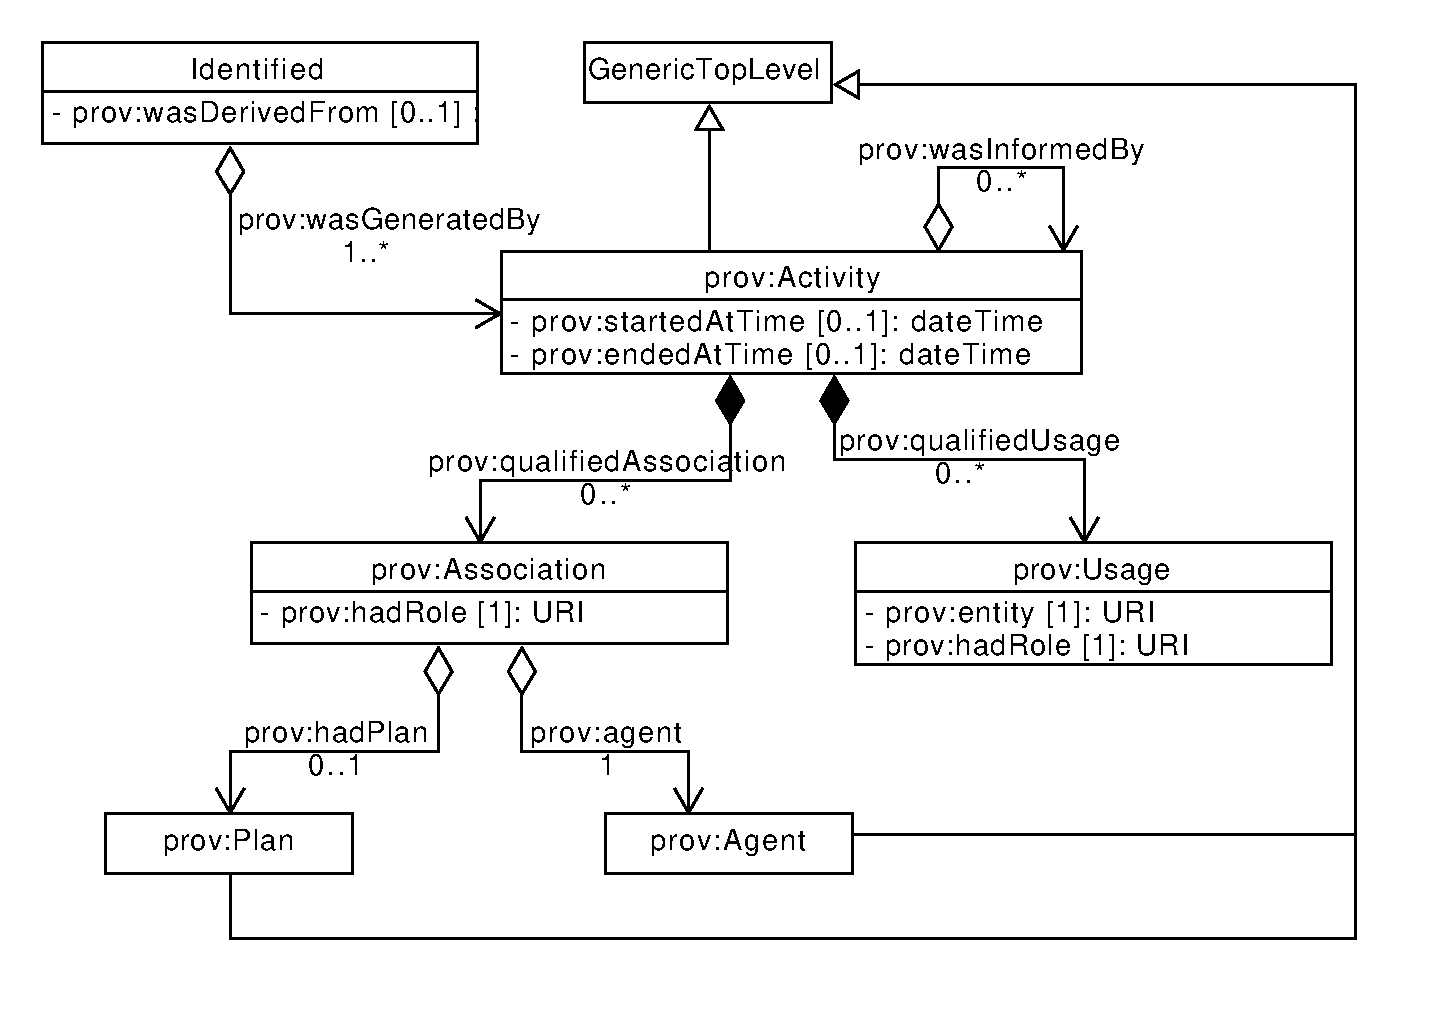
\includegraphics[scale=0.6]{uml/provenance}
\caption[]{Relationships between SBOL and PROV-O classes. The PROV-O classes \external{prov:Activity}, \external{prov:Plan}, and \external{prov:Agent} all derive from \sbol{TopLevel} in the context of the SBOL data model.
\label{uml:provenance}}
\end{center}
\end{figure}

\subsubsection{Activity}
\label{sec:prov:Activity}

A generated \texttt{Entity} is linked through a \texttt{prov:wasGeneratedBy} relationship to an \prov{Activity}, which is used to describe how different \prov{Agent}s and other entities were used. An \prov{Activity} is linked through a \prov{qualifiedUsage} to \prov{Association}s, to describe the role of agents, and is linked through \prov{qualifiedUsage} to \prov{Usage}s to describe the role of other entities used as part of the activity. Moreover, each \prov{Activity} includes optional \prov{startedAtTime} and \prov{endedAtTime} properties. When using \prov{Activity} to capture how an entity was derived, it is expected that any additional information needed will be attached as annotations. This may include software settings or textual notes. Activities can also be linked together using the \prov{wasInformedBy} relationship to provide dependency without explicitly specifying start and end times.

\subparagraph{The \sbolheading{type} property}\label{sec:types:Activity}
The \sbolmult{types:Activity}{type} property is an OPTIONAL set of \sbol{URI}s that explicitly specify the type of the provenance \prov{Activity} in more detail. If specified, it is RECOMMENDED that at least one \sbol{URI} of the \sbolmult{types:Activity}{type} property of an \prov{Activity} refers to a \sbol{URI} from \ref{tbl:activity_types}.

\subparagraph{The \sbolheading{startedAtTime} property}\label{sec:prov:startedAtTime}
The \prov{startedAtTime} property is OPTIONAL and contains a DateTime (see~\ref{sec:DateTime}) value, indicating when the activity started.  If this property is present, then the \sbol{endedAtTime} property is REQUIRED.

\subparagraph{The \sbolheading{endedAtTime} property}\label{sec:prov:endedAtTime}
The \prov{endedAtTime} property is OPTIONAL and contains a DateTime (see~\ref{sec:DateTime}) value, indicating when the activity ended.

\subparagraph{The \sbolheading{qualifiedAssociation} property}\label{sec:prov:Associations}
The \prov{qualifiedAssociation} property is OPTIONAL and MAY contain a set of \sbol{URI}s that refers to \prov{Association} objects.

\subparagraph{The \sbolheading{qualifiedUsage} property}\label{sec:prov:qualifiedUsage}
The \prov{qualifiedUsage} property is OPTIONAL and MAY contain a set of \sbol{URI}s that refers to \sbol{Usage} objects.

\subparagraph{The \sbolheading{wasInformedBy} property}\label{sec:prov:wasInformedBy}
The \prov{wasInformedBy} property is OPTIONAL and MAY contain a set of \sbol{URI}s that refers to other \prov{Activity} objects.

\subsubsection{Usage}
\label{sec:prov:Usage}
How different entities are used in an \prov{Activity} is specified with the \prov{Usage} class, which is linked from an \prov{Activity} through the \prov{Usage} relationship. A \prov{Usage} is then linked to an \texttt{Entity} through the \texttt{Entity}'s \sbol{URI} and the role of this entity is qualified with the \sbolmult{roles:U}{prov:hadRole} property. When the \prov{wasDerivedFrom} property is used together with the full provenance described here, the entity pointed at by the \prov{wasDerivedFrom} property MUST be included in a \prov{Usage}.

\subparagraph{The \sbolheading{entity} property}\label{sec:prov:entity}
The \prov{entity} property is REQUIRED and MUST contain a \sbol{URI} which MAY refer to an SBOL Identified object.

\subparagraph{The \sbolheading{hadRole} property}\label{sec:roles:U}
The \sbolmult{roles:U}{prov:hadRole} property is an OPTIONAL set of \sbol{URI}s that refer to particular term(s) describing the usage of an \prov{entity} referenced by the \prov{entity} property. Recommended terms that are defined in \ref{tbl:activity_types} can be used to indicate how the referenced \prov{entity} is being used in this \prov{Activity}.

\subsubsection{Association}
\label{sec:prov:Association}
An \prov{Association} is linked to an \prov{Agent} through the \prov{agent} relationship. The \prov{Association} includes the \sbolmult{roles:A}{prov:hadRole} property to qualify the role of the \prov{Agent} in the \prov{Activity}.

\subparagraph{The \sbolheading{agent} property}\label{sec:agent}
The \prov{agent} property is REQUIRED and MUST contain a \sbol{URI} that refers to an \prov{Agent} object.

\subparagraph{The \sbolheading{hadRole} property}\label{sec:roles:A}
The \sbolmult{roles:A}{prov:hadRole} property is an OPTIONAL set of \sbol{URI}s that refers to particular term(s) that describes the the role of the \prov{agent} in the parent \prov{Activity}. 

\subparagraph{The \sbolheading{hadPlan} property}\label{sec:plan}
The \prov{hadPlan} property is OPTIONAL and contains a \sbol{URI} that refers to a \prov{Plan}.

\subsubsection{Plan}
\label{sec:prov:Plan}

 The \prov{Plan} entity can be used as a place holder to describe the steps (for example scripts or lab protocols) taken when an \prov{Agent} is used in a particular \prov{Activity}. 

\subsubsection{Agent}
\label{sec:prov:Agent}

 Examples of agents are person, organization or software. These agents should be annotated with additional information, such as software version, needed to be able to run the same software again.

\subparagraph{Example - Codon optimization}

 Codon optimization is a practical real-wold example where provenance properties can be applied. Using the current specification, the relationship between an original CDS and the codon-optimized version could simply be represented using the \prov{wasDerivedFrom} predicate, in a light-weight form. With more comprehensive use of the PROV ontology, the codon optimization can be represented as an \prov{Activity}. This \prov{Activity} can then include additional information, such as the \prov{Agent} responsible (in this case, codon-optimizing software), and additional parameters.

\subparagraph{Example - Deriving strains}

Bacterial strains are often derived from other strains through modifications such as gene knockouts or mutations. For example, the \textit{Bacillus subtilis} 168 strain was derived from the NCIMB3610 strain in the 1940s through x-radiation. \textit{B. subtilis} 168 is a laboratory strain and has several advantages as a model organism in synthetic biology. Particularly, the 168 strain is easy to transform and is not motile, facilitating the analysis of engineered cells. The parent strain, on the other hand, is motile but more difficult to transform. The example below shows the derivation of the 168 strain using the new provenance classes.

\subparagraph{Example - Design-build-test-learn Workflow}

This particular example represents an idealized workflow for model-based design. The workflow begins with a \sbol{Model} which describes the hypothesized behavior of a biological device. Using a computational tool, a new Design (\sbol{Component}) is composed of biological parts which links back to its \sbol{Model}. A genetic construct is then produced in the laboratory via an assembly protocol, and this biological sample is represented by a Build (\sbol{Implementation}). Once constructed, the Build is then characterized in the laboratory using an automated measurement protocol on a Tecan plate reader, thus generating Test data (represented by an \sbol{ExperimentalData}). Finally, a new \sbol{Model} is derived from these data using some a fitting algorithm implemented in the Python programming language. The final \sbol{Model} may not match the beginning \sbol{Model}, as the observed behavior may not match the prediction. This example illustrates one complete iteration through a design-build-test-learn cycle, as shown in \ref{images:design-build-test-learn}.

\begin{figure}[ht]
\begin{center}
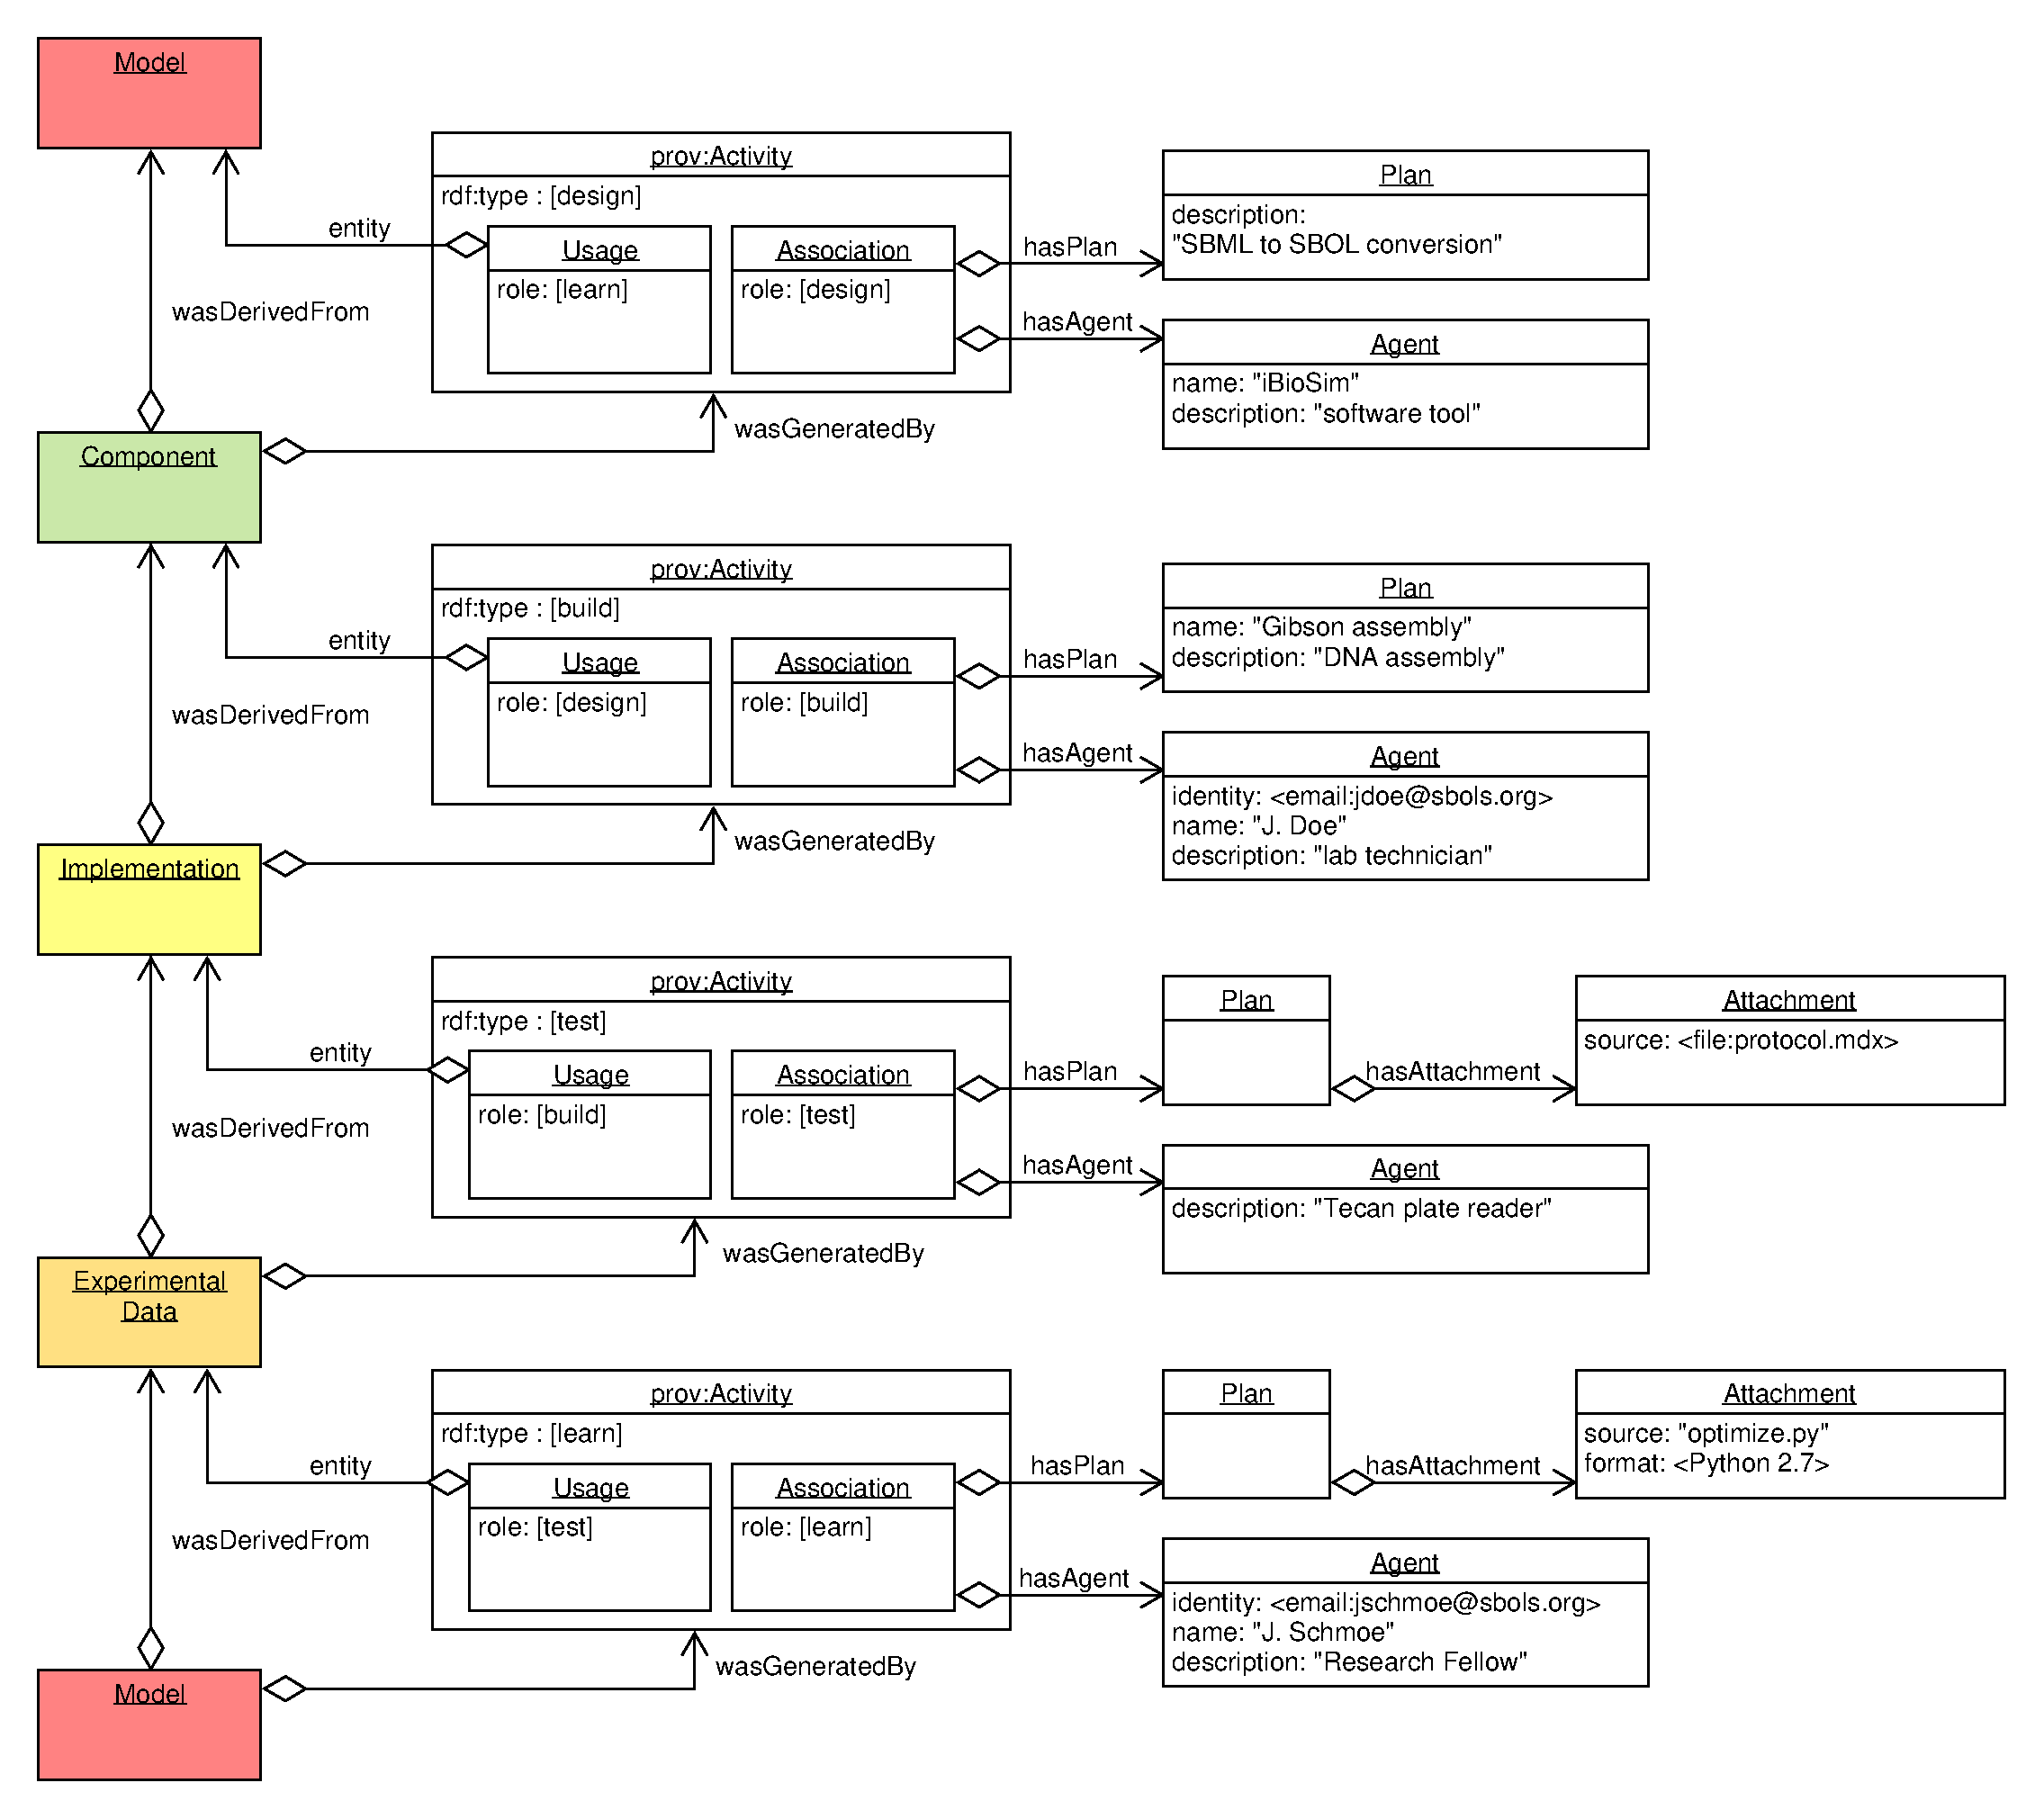
\includegraphics[width=\linewidth]{uml/design-build-test}
\caption[]{An example data structure representing an idealized workflow for model-based
design}
\label{images:design-build-test-learn}
\end{center}
\end{figure}

%% proposed by issue #137
\clearpage

\subparagraph{Example - Combinatorial Derivation}
This example illustrates how the Prov ontology should be used to reference to link a generated design to the combinatorial derivation that it was generated from.  In this example, there is a top-level derivation (Promoter\_Derivation) which specifies two possible promoters for this design, as well as an additional derivation (Terminator\_Derivation) to be used for the Gen\_Component.  The second derivation (Terminator\_Derivation) specifies two possible terminators to used within the Gen\_Component.  The derived design (Derivation\_example\_GeneratedInstance11) has a reference in the \prov{wasDerivedFrom} list to the \sbol{CombinatorialDerivation} that it was derived from (i.e., Promoter\_Derivation).  Also, each component has reference in the \prov{wasDerivedFrom} list to the component within the \sbol{template} that it is derived from.  The Gen\_Component in this derived design refers to a derived design for it (i.e., Gen\_GeneratedInstance1).  This design has a reference in the \prov{wasDerivedFrom} list that refers to the \sbol{CombinatorialDerivation} that is used to derive it (i.e., Terminator\_Derivation).  Once again, each component has a reference in the \prov{wasDerivedFrom} list to the component within the \sbol{template} that it is derived from.  The advantage of these provenance links is that they provide sufficient information to validate that this derived design has been properly derived from the specified \sbol{CombinatorialDerivation}s.

\subsection{Adding Measures/Parameters with OM}
\label{sec:parameters}

There are at least two well-established cases for including measures/parameters and their associated units in SBOL design specifications. These use cases are the specification of genetic circuit designs and their associated parameters (such as rates of transcription) and the specification of environmental conditions for biological system designs (such as growth media concentrations and temperatures). In the first use case, parameters are necessary to enable the generation of quantitive models of circuit behavior from circuit design specifications. In the second use case, measures are necessary to define experimental conditions and enable the analysis of system behavior or characterization with respect to environmental context.

The Ontology of Units of Measure (OM) (\url{http://www.ontology-of-units-of-measure.org/resource/om-2}) already defines a data model for representing measures and their associated units. Here, a subset of OM is adopted by SBOL to describe these concepts for biological design specifications. As shown in \ref{uml:om}, SBOL leverages three of the base classes defined by the OM: \om{Measure}, \om{Unit} and \om{Prefix}. A \om{Measure} links a numerical value to a \om{Unit}, which may or may not have a \om{Prefix} (e.g. centi, milli, micro, etc.). As these classes are adopted by SBOL, \om{Measure} is treated as a subclass of \sbol{Identified}, while \om{Unit} and \om{Prefix} are treated as subclasses of \sbol{TopLevel}. In addition, SBOL adopts the following OM \om{Unit} subclasses: \om{SingularUnit}, \om{CompoundUnit}, \om{UnitMultiplication}, \om{UnitDivision}, \om{UnitExponentiation}, and \om{PrefixedUnit}. Lastly, SBOL adopts the following \om{Prefix} subclasses from OM: \om{SIPrefix} and \om{BinaryPrefix}.

\begin{figure}[ht]
\begin{center}
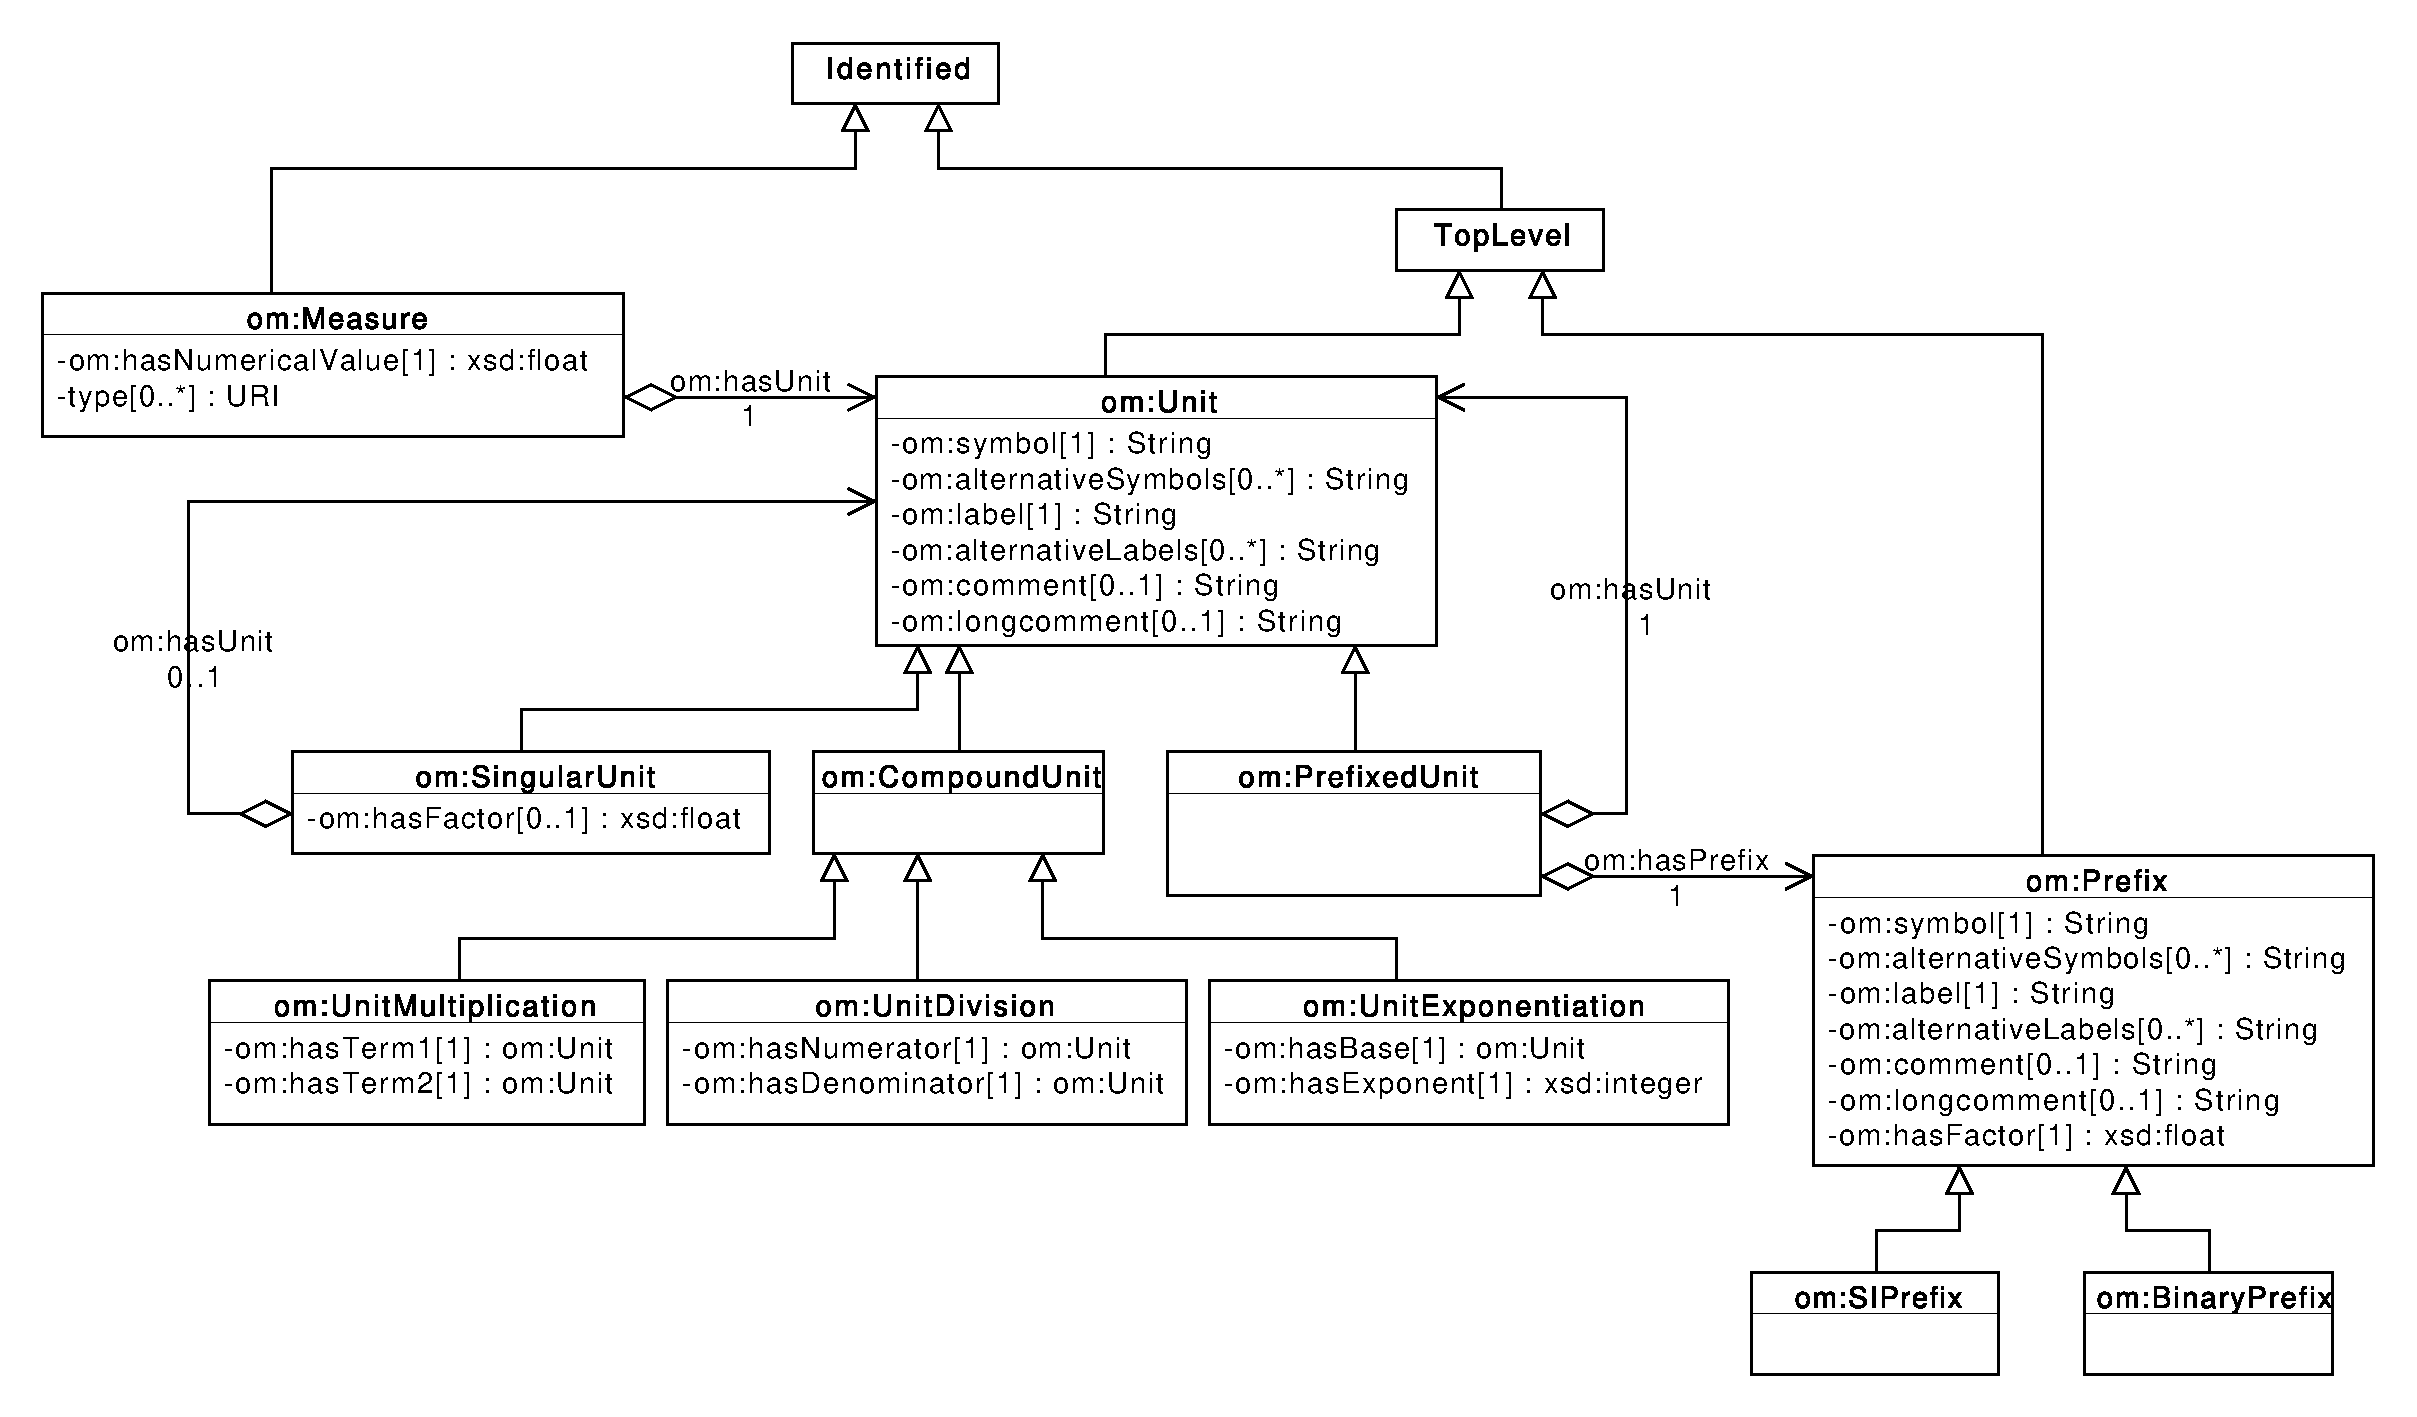
\includegraphics[width=\linewidth]{uml/om}
\caption[]{OM classes adopted by SBOL and their subclass relationships to \sbol{Identified} and \sbol{TopLevel}}
\label{uml:om}
\end{center}
\end{figure}

SBOL-compliant tools are allowed to read, write, and modify data belonging to OM classes other than those described here, but this specification does not provide any guidance for the interpretation or use of these data in the context of SBOL.

\subsubsection{Measure}
\label{sec:om:Measure}

The purpose of the \om{Measure} class is to link a numerical value to a \om{Unit}. 

\subparagraph{The \sbolheading{hasNumericalValue} property}\label{sec:hasNumericalValue}
The \sbol{hasNumericalValue} property is REQUIRED and MUST contain a single xsd:float.

\subparagraph{The \sbolheading{hasUnit} property}\label{sec:hasUnit:Measure}
The \sbolmult{hasUnit:Measure}{hasUnit} property is REQUIRED and MUST contain a \sbol{URI} that refers to a \om{Unit}. The OM provides \sbol{URI}s for many existing instances of the \om{Unit} class for reference (for example, \url{http://www.ontology-of-units-of-measure.org/resource/om-2/gramPerLitre}).

\subparagraph{The \sbolheading{types} property}\label{sec:types:Measure}
The \sbolmult{types:Measure}{types} property is OPTIONAL and MAY contain a set of \sbol{URI}s. It is RECOMMENDED that one of these \sbol{URI}s identify a term from the Systems Biology Ontology (SBO) (\url{http://www.ebi.ac.uk/sbo/main/}). This \sbolmult{types:Measure}{types} property of the \om{Measure} class is not specified in the OM and is added by SBOL to describe different types of parameters (for example, rate of reaction is identified by the SBO term \url{http://identifiers.org/biomodels.sbo/SBO:0000612}).

\subsubsection{Unit}
\label{sec:om:Unit}

As adopted by SBOL, \om{Unit} is an abstract class that is extended by other classes to describe units of measure using a shared set of properties. 

\subparagraph{The \sbolheading{symbol} property}\label{sec:symbol:Unit}
The \sbolmult{symbol:Unit}{symbol} property is REQUIRED and MUST contain a \sbol{String}. This \sbol{String} is commonly used to abbreviate the unit of measure's name. For example, the unit of measure named ``gram per liter'' is commonly abbreviated using the \sbol{String} ``g/l''.

\subparagraph{The \sbolheading{alternativeSymbols} property}\label{sec:alternativeSymbols:Unit}
The \sbolmult{alternativeSymbols:Unit}{alternativeSymbols} property is OPTIONAL and MAY contain a set of \sbol{String}s. This property can be used to specify alternative abbreviations other than that specified using the \sbolmult{symbol:Unit}{symbol} property.

\subparagraph{The \sbolheading{label} property}\label{sec:label:Unit}
The \sbolmult{label:Unit}{label} property is REQUIRED and MUST contain a \sbol{String}. This \sbol{String} is a common name for the unit of measure and SHOULD be identical to any \sbol{String} contained by the \sbol{name} property inherited from \sbol{Identified}.

\subparagraph{The \sbolheading{alternativeLabels} property}\label{sec:alternativeLabels:Unit}
The \sbolmult{alternativeLabels:Unit}{alternativeLabels} property is OPTIONAL and MAY contain a set of \sbol{String}s. This property can be used to specify alternative common names other than that specified using the \sbolmult{label:Unit}{label} property.

\subparagraph{The \sbolheading{comment} property}\label{sec:comment:Unit}
The \sbolmult{comment:Unit}{comment} property is OPTIONAL and MAY contain a \sbol{String}. This \sbol{String} is a description of the unit of measure and SHOULD be identical to any \sbol{String} contained by the \sbol{description} property inherited from \sbol{Identified}.

\subparagraph{The \sbolheading{longcomment} property}\label{sec:longcomment:Unit}
The \sbolmult{longcomment:Unit}{longcomment} property is OPTIONAL and MAY contain a \sbol{String}. This \sbol{String} is a long description of the unit of measure and SHOULD be longer than any \sbol{String} contained by the \sbolmult{comment:Unit}{comment} property.

\subsubsection{SingularUnit}
\label{sec:om:SingularUnit}

The purpose of the \om{SingularUnit} class is to describe a unit of measure that is not explicitly represented as a combination of multiple units, but could be equivalent to such a representation. For example, a joule is considered to be a \om{SingularUnit}, but it is equivalent to the multiplication of a newton and a meter.  

\subparagraph{The \sbolheading{hasUnit} property}\label{sec:hasUnit:SingularUnit}
The \sbolmult{hasUnit:SingularUnit}{hasUnit} is OPTIONAL and MAY contain a \sbol{URI}. This \sbol{URI} MUST refer to another \om{Unit}. The \sbolmult{hasUnit:SingularUnit}{hasUnit} propery can be used in conjunction with the \sbolmult{hasFactor:SingularUnit}{hasFactor} property to specify whether a \om{SingularUnit} is equivalent to another \om{Unit} multiplied by a factor. For example, an angstrom is equivalent to $10^{-10}$ meters.

\subparagraph{The \sbolheading{hasFactor} property}\label{sec:hasFactor:SingularUnit}
The \sbolmult{hasFactor:SingularUnit}{hasFactor} property is OPTIONAL and MAY contain a xsd:float. If the \sbolmult{hasFactor:SingularUnit}{hasFactor} property of a \om{SingularUnit} is non-empty, then its \sbolmult{hasUnit:SingularUnit}{hasUnit} property SHOULD also be non-empty.

\subsubsection{CompoundUnit}
\label{sec:om:CompoundUnit}

As adopted by SBOL, \om{CompoundUnit} is an abstract class that is extended by other classes to describe units of measure that can be represented as combinations of multiple other units of measure.

\subsubsection{UnitMultiplication}
\label{sec:om:UnitMultiplication}

The purpose of the \om{UnitMultiplication} class is to describe a unit of measure that is the multiplication of two other units of measure. 

\subparagraph{The \sbolheading{hasTerm1} property}\label{sec:hasTerm1}
The \sbol{hasTerm1} property is REQUIRED and MUST contain a \sbol{URI} that refers to another \om{Unit}. This \om{Unit} is the first multiplication term.

\subparagraph{The \sbolheading{hasTerm2} property}\label{sec:hasTerm2}
The \sbol{hasTerm2} property is REQUIRED and MUST contain a \sbol{URI} that refers to another \om{Unit}. This \om{Unit} is the second multiplication term. It is okay if the \om{Unit} referred to by \sbol{hasTerm1} is the same as that referred to by \sbol{hasTerm2}.

\subsubsection{UnitDivision}
\label{sec:om:UnitDivision}

The purpose of the \om{UnitDivision} class is to describe a unit of measure that is the division of one unit of measure by another.

\subparagraph{The \sbolheading{hasNumerator} property}\label{sec:hasNumerator}
The \sbol{hasNumerator} property is REQUIRED and MUST contain a \sbol{URI} that refers to another \om{Unit}.

\subparagraph{The \sbolheading{hasDenominator} property}\label{sec:hasDenominator}
The \sbol{hasDenominator} property is REQUIRED and MUST contain a \sbol{URI} that refers to another \om{Unit}.

\subsubsection{UnitExponentiation}
\label{sec:om:UnitExponentiation}

The purpose of the \om{UnitExponentiation} class is to describe a unit of measure that is raised to an integer power.

\subparagraph{The \sbolheading{hasBase} property}\label{sec:hasBase}
The \sbol{hasBase} property is REQUIRED and MUST contain a \sbol{URI} that refers to another \om{Unit}.

\subparagraph{The \sbolheading{hasExponent} property}\label{sec:hasExponent}
The \sbol{hasExponent} property is REQUIRED and MUST contain an \texttt{xsd:integer}.

\subsubsection{PrefixedUnit}
\label{sec:om:PrefixedUnit}

The purpose of the \om{PrefixedUnit} class is to describe a unit of measure that is the multiplication of another unit of measure and a factor represented by a standard prefix such as ``milli,'' ``centi,'' ``kilo,'' etc. 

\subparagraph{The \sbolheading{hasUnit} property}\label{sec:hasUnit:PrefixedUnit}
The \sbolmult{hasUnit:PrefixedUnit}{hasUnit} property is REQUIRED and MUST contain a \sbol{URI} that refers to another \om{Unit}. 

\subparagraph{The \sbolheading{hasPrefix} property}\label{sec:hasPrefix}
The \sbol{hasPrefix} property is REQUIRED and MUST contain a \sbol{URI} that refers to a \om{Prefix}.

\subsubsection{Prefix}
\label{sec:om:Prefix}

As adopted by SBOL, \om{Prefix} is an abstract class that is extended by other classes to describe factors that are commonly represented by standard unit prefixes. For example, the factor $10^{-3}$ is represented by the standard unit prefix ``milli.'' 

\subparagraph{The \sbolheading{symbol} property}\label{sec:symbol:Prefix}
The \sbolmult{symbol:Prefix}{symbol} property is REQUIRED and MUST contain a \sbol{String}. This \sbol{String} is commonly used to abbreviate the name of the unit prefix. For example, the \sbol{String} ``m'' is commonly used to abbreviate the name ``milli.''

\subparagraph{The \sbolheading{alternativeSymbols} property}\label{sec:alternativeSymbols:Prefix}
The \sbolmult{alternativeSymbols:Prefix}{alternativeSymbols} property is OPTIONAL and MAY contain a set of \sbol{String}s. This property can be used to specify alternative abbreviations other than that specified using the \sbolmult{symbol:Prefix}{symbol} property.

\subparagraph{The \sbolheading{label} property}\label{sec:label:Prefix}
The \sbolmult{label:Prefix}{label} property is REQUIRED and MUST contain a \sbol{String}. This \sbol{String} is a common name for the unit prefix and SHOULD be identical to any \sbol{String} contained by the \sbol{name} property inherited from \sbol{Identified}.

\subparagraph{The \sbolheading{alternativeLabels} property}\label{sec:alternativeLabels:Prefix}
The \sbolmult{alternativeLabels:Prefix}{alternativeLabels} property is OPTIONAL and MAY contain a set of \sbol{String}s. This property can be used to specify alternative common names other than that specified using the \sbolmult{label:Prefix}{label} property.

\subparagraph{The \sbolheading{comment} property}\label{sec:comment:Prefix}
The \sbolmult{comment:Prefix}{comment} property is OPTIONAL and MAY contain a \sbol{String}. This \sbol{String} is a description of the unit prefix and SHOULD be identical to any \sbol{String} contained by the \sbol{description} property inherited from \sbol{Identified}.

\subparagraph{The \sbolheading{longcomment} property}\label{sec:longcomment:Prefix}
The \sbolmult{longcomment:Prefix}{longcomment} property is OPTIONAL and MAY contain a \sbol{String}. This \sbol{String} is a long description of the unit of measure and SHOULD be longer than any \sbol{String} contained by the \sbolmult{comment:Prefix}{comment} property.

\subparagraph{The \sbolheading{hasFactor} property}\label{sec:hasFactor:Prefix}
The \sbolmult{hasFactor:Prefix}{hasFactor} property is REQUIRED and MUST contain an xsd:float.

\subsubsection{SIPrefix}
\label{sec:om:SIPrefix}

The purpose of the \om{SIPrefix} class is to describe standard SI prefixes such as ``milli,'' ``centi,'' ``kilo,'' etc. 


\subsubsection{BinaryPrefix}
\label{sec:om:BinaryPrefix}

The purpose of the \om{BinaryPrefix} class is to describe standard binary prefixes such as ``kibi,'' ``mebi,'' ``gibi,'' etc. These prefixes commonly precede units of information such as ``bit'' and ``byte.''

\begin{figure}[ht]
\begin{center}
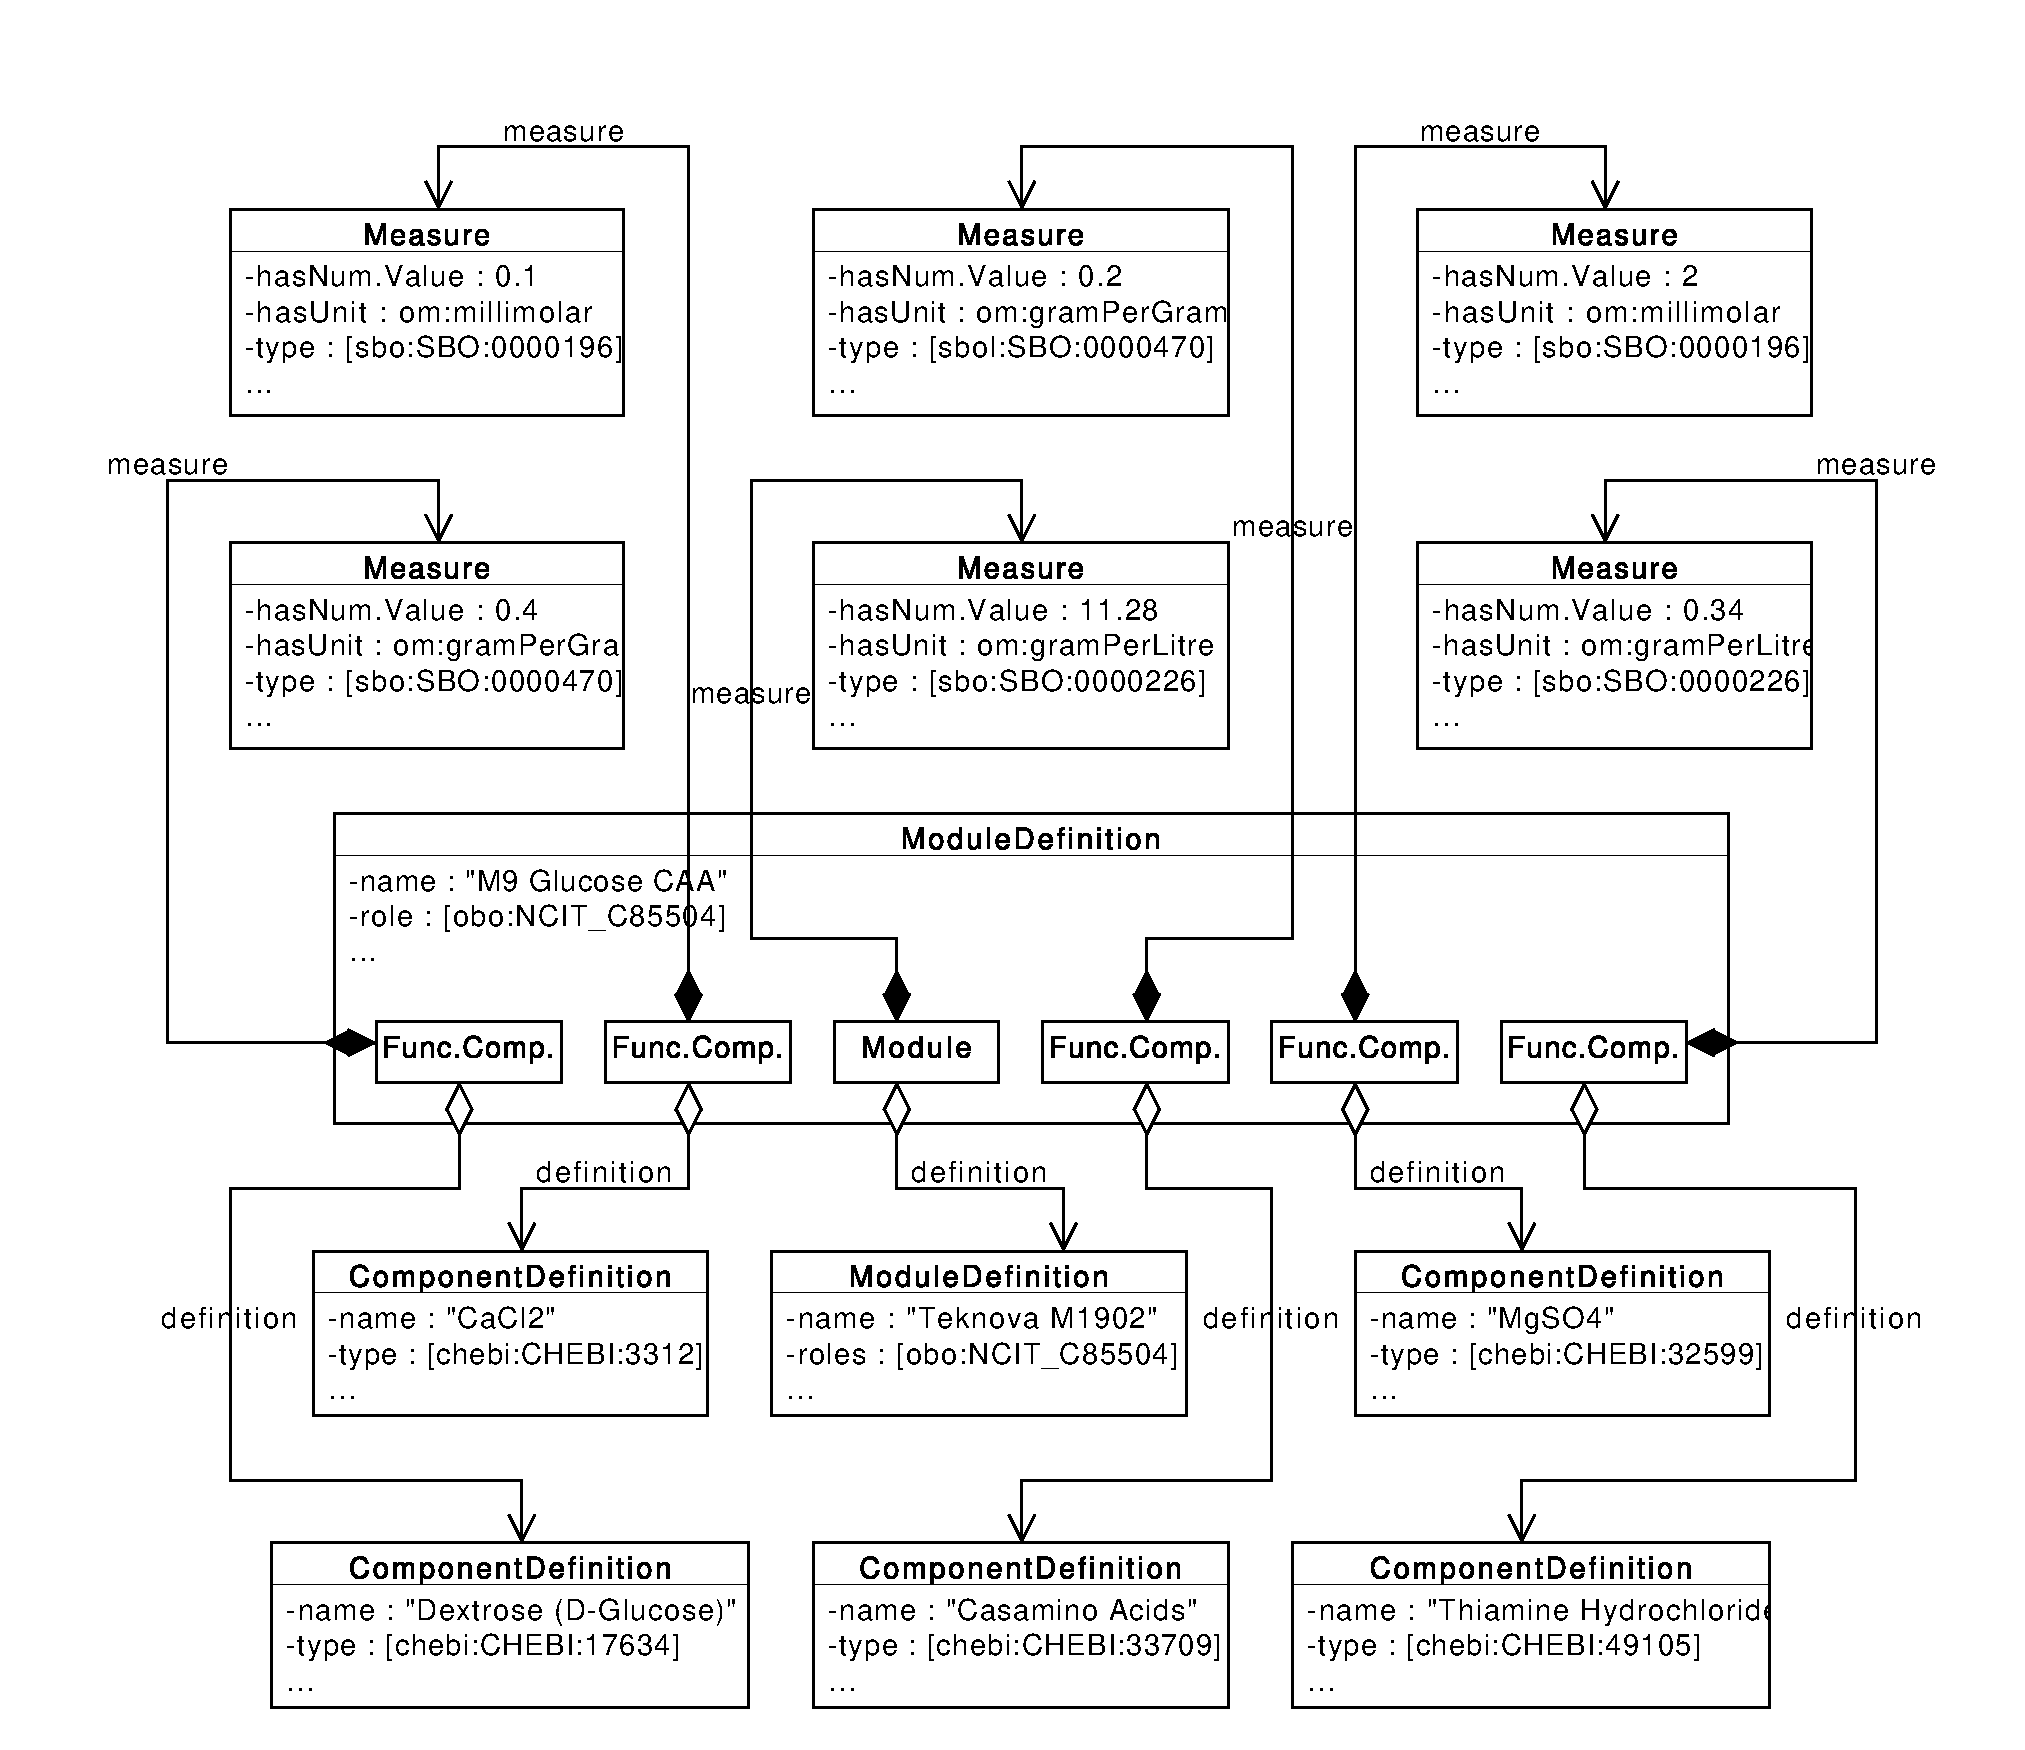
\includegraphics[width=\linewidth]{uml/media_example}
\caption[]{Growth media recipe represented using instances of the \om{Measure} and \om{Unit} classes from the OM.}
\label{uml:media_example}
\end{center}
\end{figure}
